\subsection{Report of 21 October 2026: ensembles and full distributions}\label{sec:w1021}

\textbf{Summary.} Two questions from Professor Shasha: can an ensemble of the models we have, or can obtain, do better; and can the models give a distribution for the margin and the total, compared with the Vegas lines.

\subsubsection{Can an ensemble do better?}

Professor Shasha asked whether an ensemble of the models we have, or can obtain, improves on them. We stacked by least squares, fitting weights on earlier seasons' out-of-sample predictions and applying them to the next season, 2013--2025. To our three models we added two public forecasts, nfelo~\cite{nfelo} (a public Elo variant with a quarterback adjustment; we use its rating difference before any regression toward the market) and FiveThirtyEight's Elo (available to 2020), and the sportsbook \emph{opening} line, which the nfelo files carry (Table~\ref{tab:ensemble}, Figure~\ref{fig:ensemble}).

\begin{table}[H]
\centering
\small
\begin{tabular}{lcp{6cm}}
\toprule
\textbf{Forecast} & \textbf{Margin MAE} & \textbf{Note} \\
\midrule
Random forest (ours) & 10.22 & \\
Ridge (ours) & 10.20 & \\
Elo (ours) & 10.25 & \\
Stack of our three & 10.18 & weights 0.19 / 0.36 / 0.51 \\
nfelo, pure model & 10.01 & history back-computed with the current model, so optimistic \\
Stack: ours + nfelo & 10.04 & our models receive weight near 0 \\
Opening line & 10.02 & \\
Closing line & 9.92 & \\
Stack: ours + nfelo + closing line & 9.95 & closing line 0.58, nfelo 0.72, ours near 0 \\
\bottomrule
\end{tabular}
\caption{Stacking test, home margin, 2013--2025 (3,562 games with all forecasts available).}
\label{tab:ensemble}
\end{table}

\begin{figure}[H]
\centering
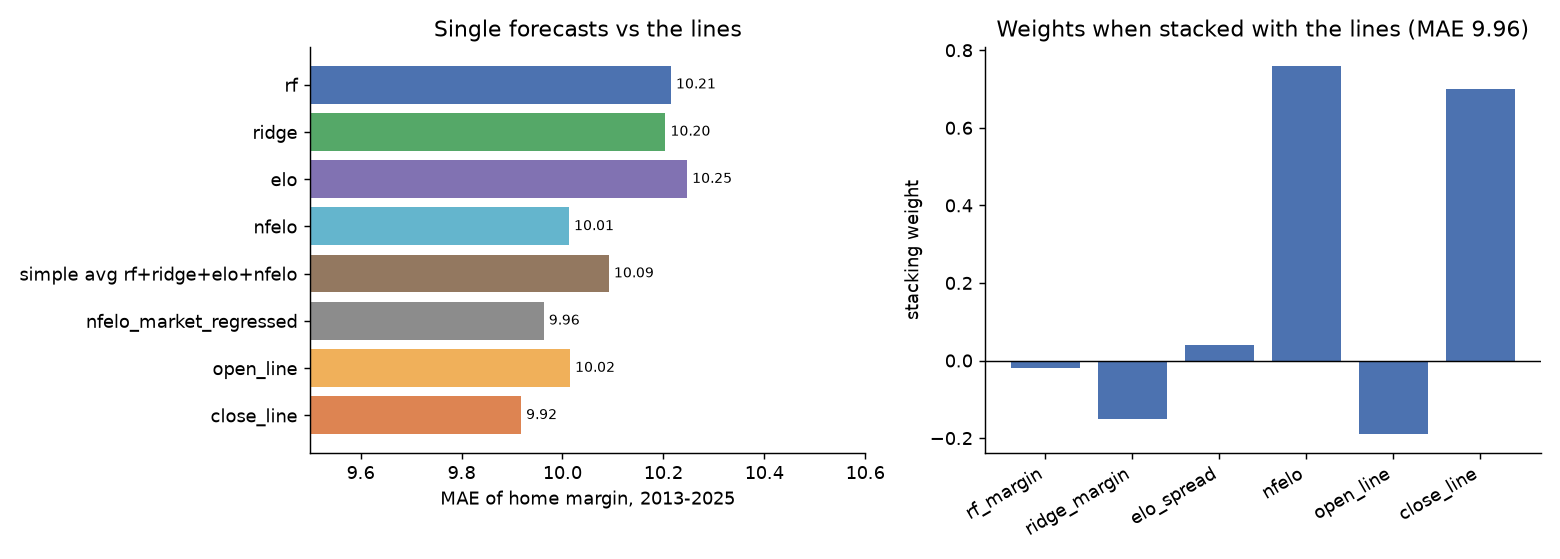
\includegraphics[width=0.98\textwidth]{ensemble_external.png}
\caption{Left: single forecasts and the lines. Right: stacking weights when our models, nfelo and both lines are combined.}
\label{fig:ensemble}
\end{figure}

Averaging our own models gains only a few hundredths of a point, because their predictions are correlated at 0.89--0.94. nfelo is a better single forecast than anything we built, by about 0.2 points, which we attribute to its quarterback adjustment and to its published history being generated by the current version of the model. Most important, no stack improves on the closing line: whenever the line is a component it takes nearly all the weight. The same holds for totals, where the opening total (10.47) is in fact slightly better than the closing total (10.53) in this sample. Ensembling what we have does not beat the market; an ensemble that could would need forecasts carrying information the market does not yet have.

\subsubsection{Full distributions and the Vegas lines}

The second question was whether the models can give a distribution for the margin and the total and how it compares with the lines. The two predicted scores set the centre, and the distribution around them comes either from the bivariate normal with the residual covariance or from the empirical grid tilted so that its mean margin and total match the forest (Figure~\ref{fig:gamedist}). From either, the probability of any outcome is a sum: $P(\text{home wins})$, $P(\text{home covers the spread})$, $P(\text{over the total})$.

\begin{figure}[H]
\centering
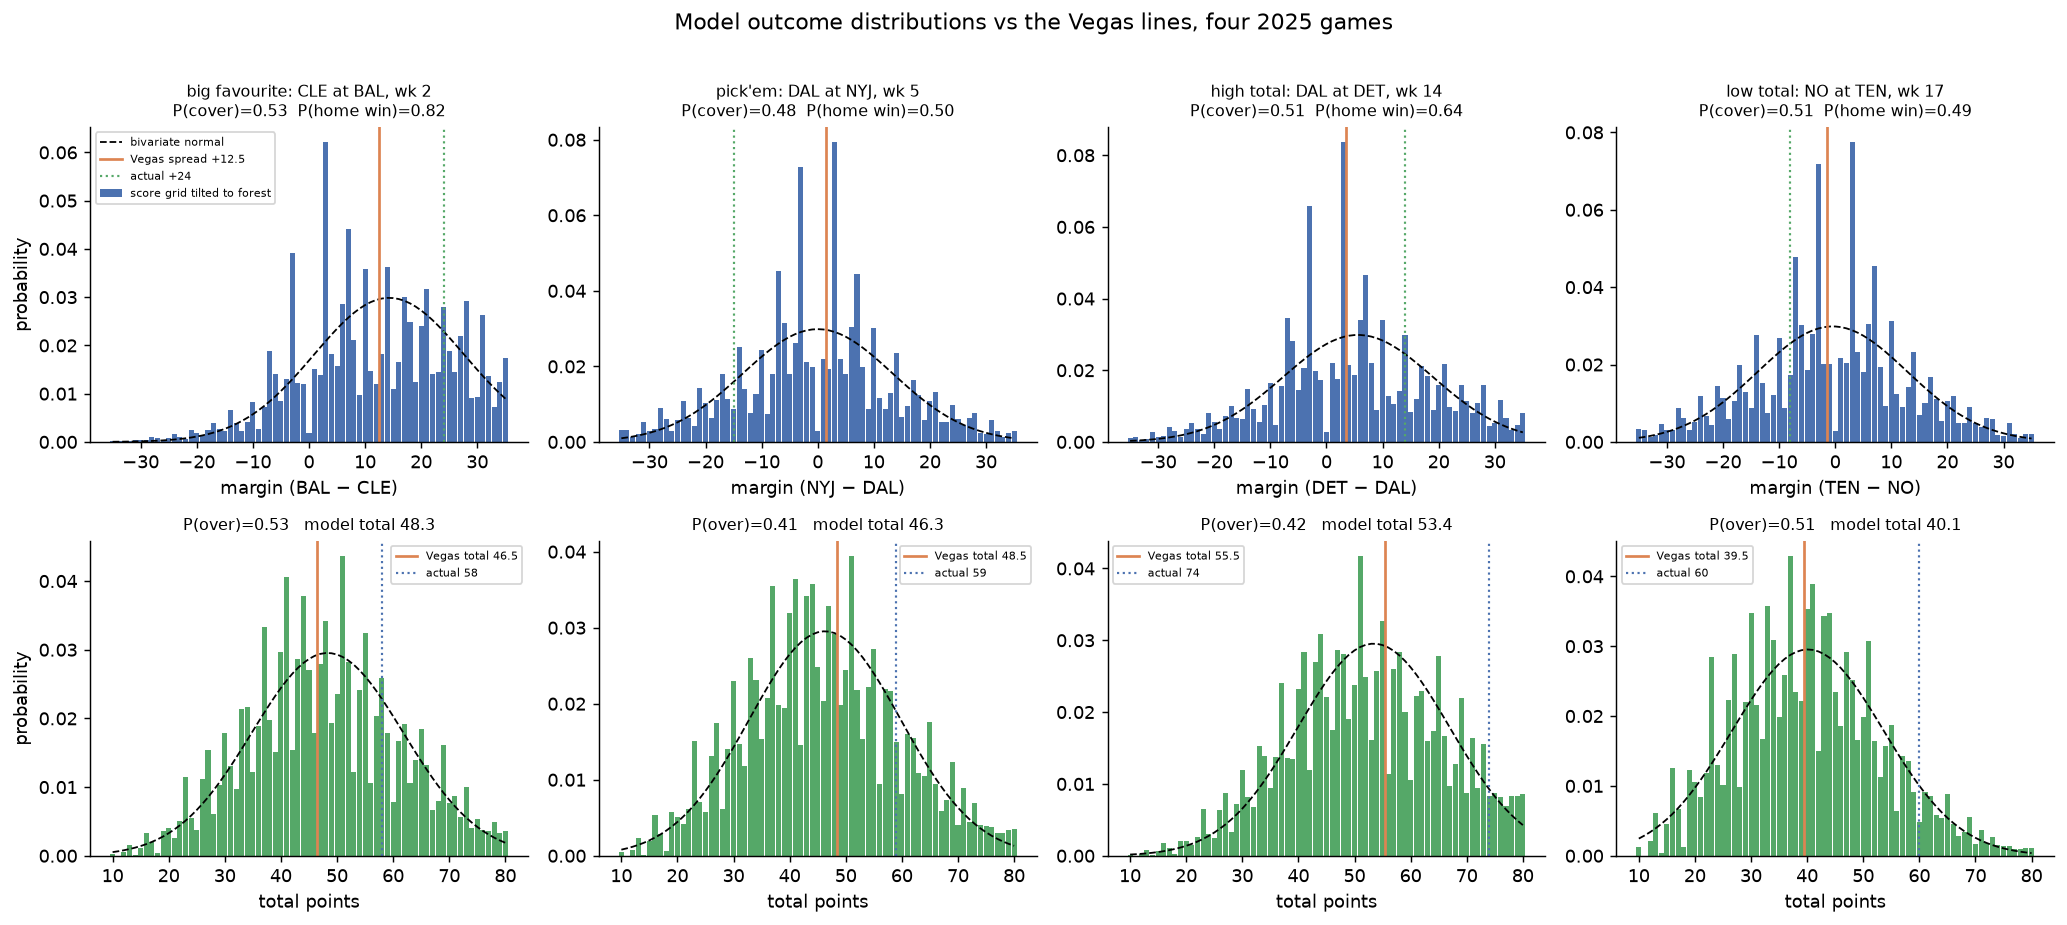
\includegraphics[width=\textwidth]{game_distributions.png}
\caption{Four 2025 games. Top: margin distribution from the tilted score grid (bars) and the bivariate normal (dashed), with the Vegas spread (orange) and the actual margin (dotted). Bottom: the same for the total.}
\label{fig:gamedist}
\end{figure}

\paragraph{How the calibration is measured.} For every game of 2016--2025 the empirical grid, with its prior built from the seasons before the test season, is tilted so that its mean margin and total equal the forest's two predictions; the model's probability of an event is the mass of that grid on the event's region. Games are then grouped by predicted probability in bins of width 0.1, and the observed frequency of the event in each bin is plotted against the mean prediction (Figures~\ref{fig:coverover} and~\ref{fig:fixedcal}). A forecast is calibrated if the points lie on the diagonal; it is informative if the predictions spread out along it. The Brier score summarises both, and we compare it with the climatological forecast that assigns every game the base rate.

\paragraph{Thresholds set by the market.} Across all 2,758 games the model's $P(\text{cover})$ averages 0.50 with a standard deviation of 0.09 and $P(\text{over})$ averages 0.49 with a standard deviation of 0.08; only a quarter of games get a cover probability outside 0.40--0.60. The calibration of these probabilities against outcomes is flat (Figure~\ref{fig:coverover}): when the model says 65\% to cover, teams cover about 52\%, and the regression slope of outcome on prediction is 0.06 for cover and 0.11 for over. Brier scores of 0.257 for cover and 0.255 for over are slightly worse than the 0.250 of the base rate. So, relative to the threshold the market has chosen, the model's probabilities carry no information. This is not a failure of calibration in the usual sense; it is what an efficient line implies. The closing spread is the market's median for the margin, set with everything the market knows, so conditioning on it removes exactly the part of the model's information that the market already has, and what remains is noise.

{\color{red}\textbf{Amine comment:} Please clarify how calibration is done. When the model predicts a 65\% chance of covering, the observed rate is about 52\%. Please also test fixed thresholds chosen in advance, separately from thresholds set by the market.}

{\color{blue}\textbf{Sai comment:} Fixed. The paragraph ``How the calibration is measured'' above states the procedure. The paragraph ``Thresholds fixed in advance'' below, with Table~\ref{tab:fixedcal} and Figure~\ref{fig:fixedcal}, tests seven pre-chosen events: the model has 8--11\% Brier skill on margin events and 3--4\% on totals with slopes 1.13--1.27, against slopes of 0.06--0.11 at the market's thresholds.}

\begin{figure}[H]
\centering
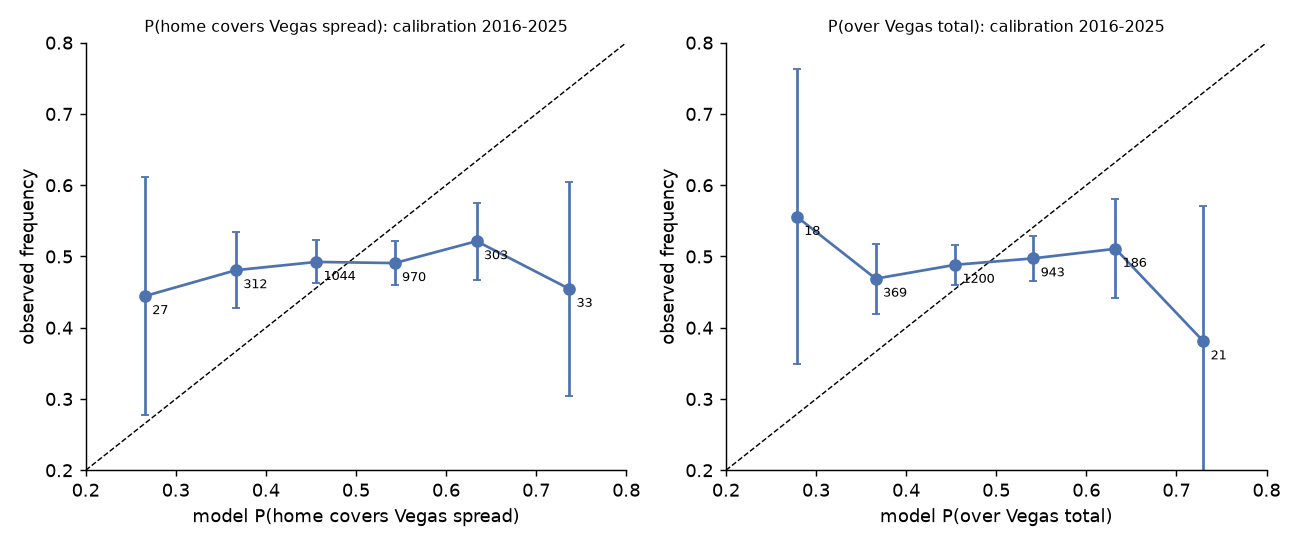
\includegraphics[width=0.95\textwidth]{cover_over_calibration.png}
\caption{Calibration of the model's cover and over probabilities against the closing line, 2016--2025; bin sizes shown.}
\label{fig:coverover}
\end{figure}

\paragraph{Thresholds fixed in advance.} The test Professor Amine asked for separates the two questions. We fixed seven thresholds before looking at the data, chosen to sit at round numbers and key numbers rather than at any game's line: the home team wins; wins by more than 3; by more than 7; the away team wins by more than 3; and the total exceeds 41, 45 and 48. For each the model probability is read from the same tilted grid, and the outcome is scored against the same 2,761 games (Table~\ref{tab:fixedcal}, Figure~\ref{fig:fixedcal}). At every fixed threshold the probabilities are informative: the Brier score beats the base rate by 8--11\% on the margin thresholds and 3--4\% on the totals, and the predictions spread across a range of 0.2 to 0.8. They are close to calibrated, with a regression slope of outcome on prediction between 1.13 and 1.27: the model is slightly under-confident, pushing its probabilities toward one half a little more than the outcomes warrant, which is the usual behaviour of a forest with large leaves. The totals carry less information than the margins (the predictions have a standard deviation of 0.08 against 0.13), consistent with the point-error table, where the model's total is further behind the line than its margin.

\begin{table}[H]
\centering
\small
\begin{tabular}{lcccccc}
\toprule
\textbf{Event} & \textbf{Base rate} & \textbf{SD of $p$} & \textbf{Brier} & \textbf{Brier, base rate} & \textbf{Skill} & \textbf{Slope} \\
\midrule
Home wins & 0.550 & 0.132 & 0.2212 & 0.2475 & 10.6\% & 1.25 \\
Home wins by $>3$ & 0.424 & 0.131 & 0.2182 & 0.2442 & 10.7\% & 1.27 \\
Home wins by $>7$ & 0.303 & 0.122 & 0.1915 & 0.2111 & 9.3\% & 1.18 \\
Away wins by $>3$ & 0.332 & 0.122 & 0.2032 & 0.2219 & 8.4\% & 1.13 \\
Total $>41$ & 0.595 & 0.076 & 0.2330 & 0.2409 & 3.3\% & 1.20 \\
Total $>45$ & 0.481 & 0.079 & 0.2406 & 0.2497 & 3.6\% & 1.24 \\
Total $>48$ & 0.396 & 0.077 & 0.2312 & 0.2391 & 3.3\% & 1.16 \\
\midrule
Home covers the closing spread & 0.493 & 0.088 & 0.2568 & 0.2499 & $-2.8\%$ & 0.06 \\
Over the closing total & 0.490 & 0.080 & 0.2550 & 0.2499 & $-2.0\%$ & 0.11 \\
\bottomrule
\end{tabular}
\caption{Model probabilities from the tilted grid scored against outcomes, 2016--2025 (2,761 games; ties excluded where they occur). Skill is one minus the ratio of the Brier score to that of the base-rate forecast; slope is the least-squares slope of the outcome on the prediction, 1 for a calibrated forecast.}
\label{tab:fixedcal}
\end{table}

\begin{figure}[H]
\centering
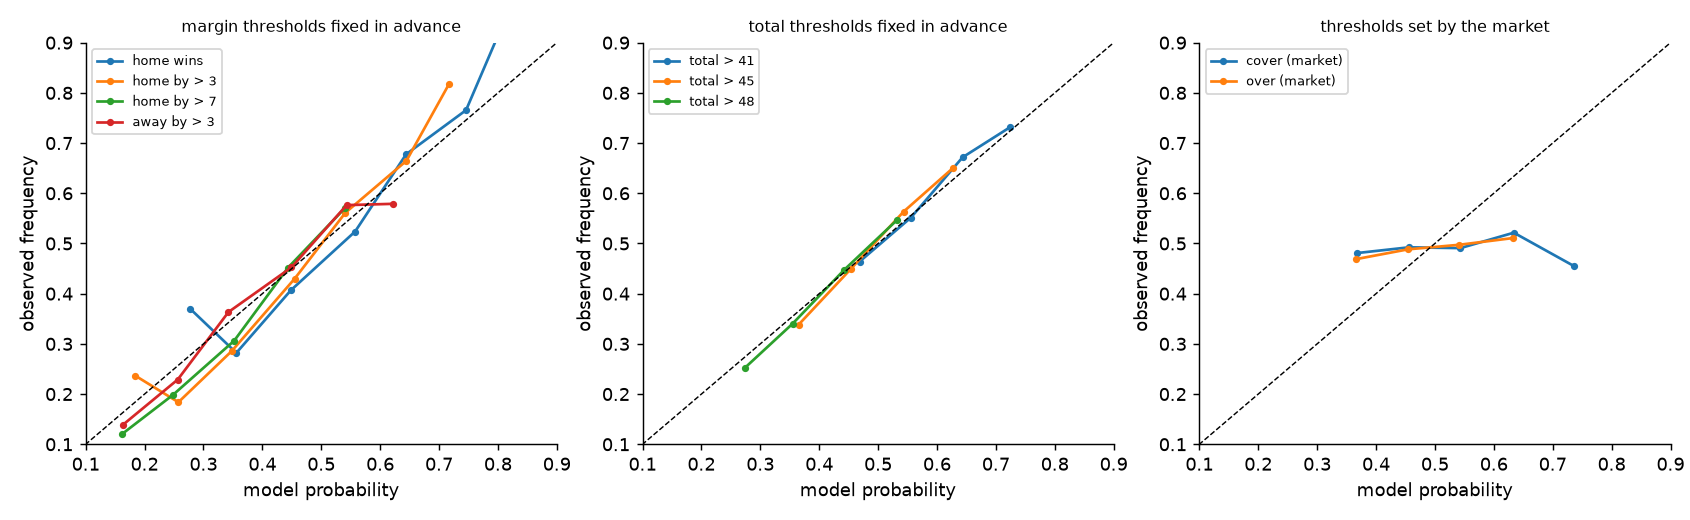
\includegraphics[width=\textwidth]{fixed_threshold_calibration.png}
\caption{Reliability of the model's probabilities at thresholds fixed in advance (left, centre) and at the thresholds set by the market (right), 2016--2025; bins with at least 30 games.}
\label{fig:fixedcal}
\end{figure}

The two tests together give the clean statement. The distributions are calibrated and informative for any event defined in advance, and carry nothing beyond what the closing line already contains for the event the line defines. The engine's value therefore lies in pricing the whole distribution consistently, not in picking sides against the market.
